\question Q4\droppoints

\begin{solution}
(a)
    Implemented.

    (b) The histogram is as follows:

    \centerline{
        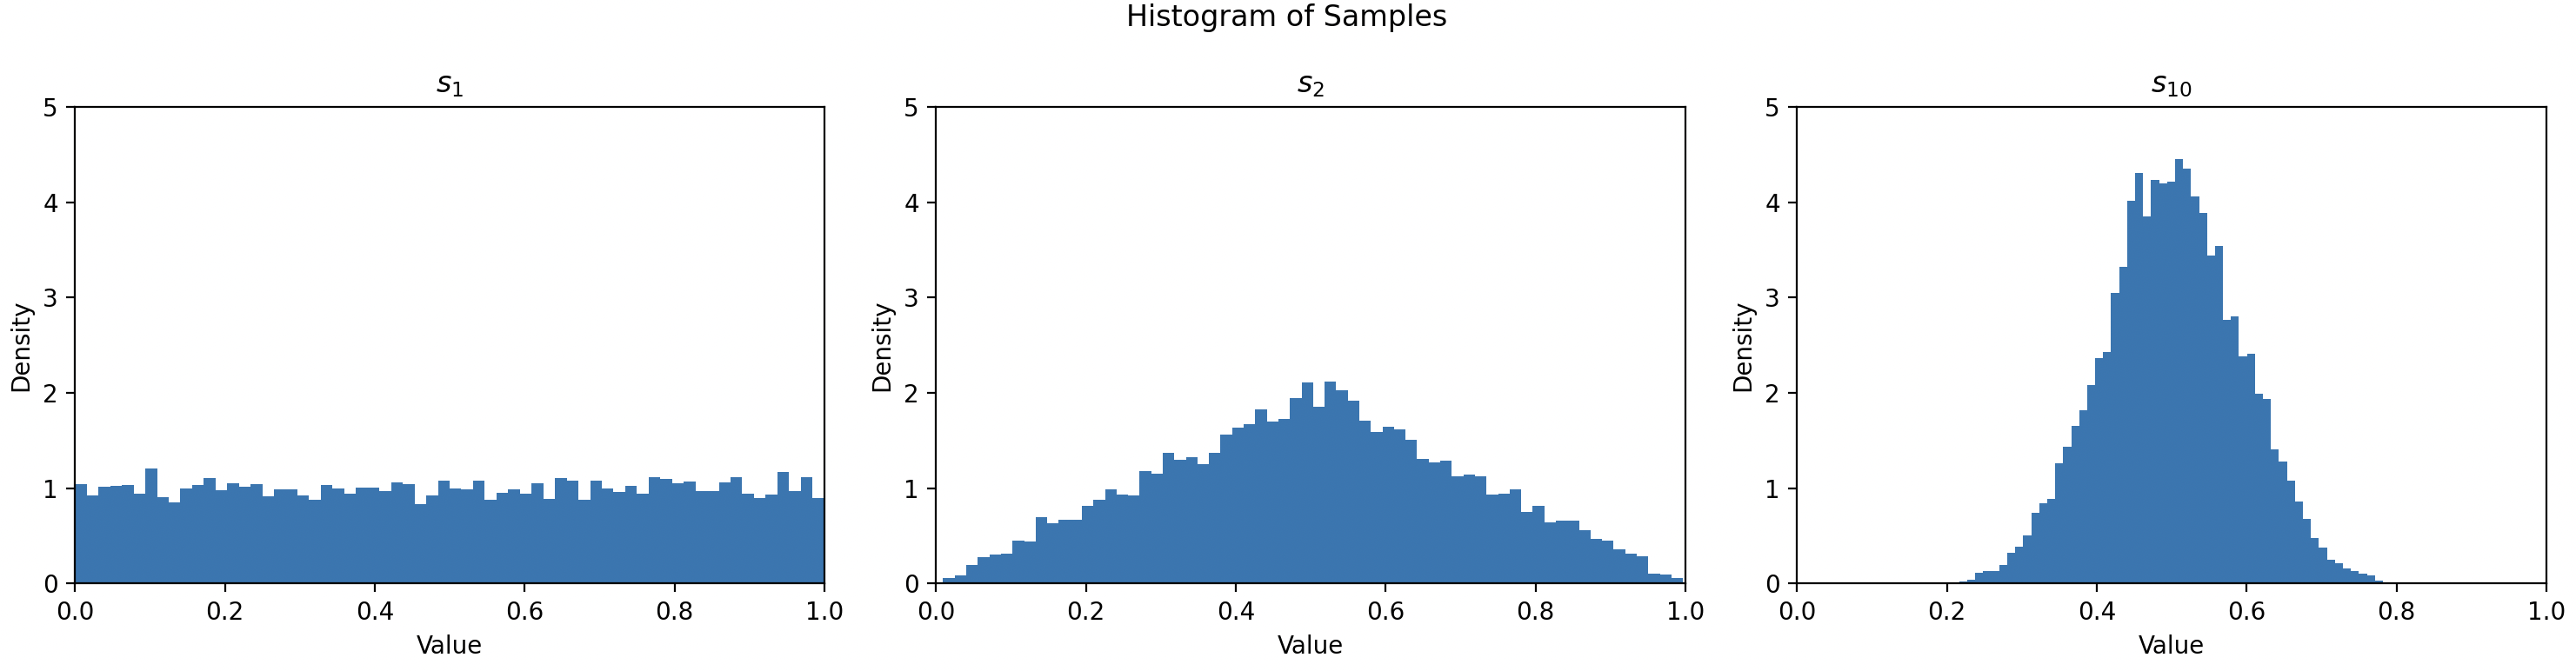
\includegraphics[width=0.75\textwidth]{img/histogram}
    }

    (c) The $s_1$ shows the PDF of uniform distribution $\mathcal{U}(0, 1)$ as expected.
    The $s_2$ shows the convolution function of the PDF of two identical PDF of uniform distribution.

    As we average more sets of samples, we observe that a progression from a uniform distribution toward a normal distribution $\mathcal{N}(0.5, \sigma^2)$.
    This is a demonstration of the Central Limit Theorem, which says that \textbf{the sampling distribution of the mean will always be normally distributed, as long as the sample size is large enough}.


\end{solution}